\documentclass[12pt]{article}

\usepackage{fullpage}
\usepackage{graphicx, rotating, booktabs} 
\usepackage{times} 
\usepackage{natbib} 
\usepackage{indentfirst} 
\usepackage{setspace}
\usepackage{grffile} 
\usepackage{hyperref}
\usepackage{adjustbox}
\usepackage{amsmath}
\setcitestyle{aysep{}}


\singlespace
\title{\textbf{Alliance Participation and Military Spending}}
\author{Joshua Alley\footnote{Graduate Student,
Department of Political Science, Texas A\&M University.}}
\date{{\normalsize \today}}

\bibliographystyle{apsr}

\begin{document}

\maketitle 

\newpage 

\doublespace 

\begin{abstract}



\end{abstract}



\section{Introduction}


How does alliance participation affect military spending? 
Previous scholarship on this issue is divided between two competing camps. 
One group expects alliance participation to reduce military spending. 
The other expects alliance members will spend more on defense. 


In this paper, I address the division between these two perspectives on alliance participation and military expenditures. 
Answering this question makes theoretical and empirical contributions. 
In my argument, I show when alliance participation increases and decreases military spending. 
Major and non-major power states use alliances for different purposes, so they respond differently to changes in treaty strength.


Major powers use strong treaty commitments to increase their influence. 
Strong treaties replace military spending as a source of influence, allowing large states to reduce spending. 
Non-major powers emphasize security from alliances, but also have high opportunity costs of military spending.  
Given a strong treaty commitment, these small states cannot reduce military spending without damaging the treaty. 
Weaker treaties still provide some security without tying military support to other costly commitments, allowing non-major powers to reduce military spending. 


I test these predictions with a novel research design.
First, I develop a latent measure of alliance treaty strength. 
Then, I employ that measure in a multilevel model which directly compares alliance treaties, and estimates the impact of each treaty on members' military spending.  


% why you should care
Unifying scholarship on alliance participation and military spending has academic and practical value.
Scholarship on this issue has paid little attention to differences between alliances.\footnote{See \citet{DigiuseppePoast2016} for an important exception.} 
As a result, we are left with competing assertions about the characteristics of alliances. 


These arguments are a poor guide for policy discussions. 
Policy debates emphasize reduced spending by alliance members- especially US allies. 
But these debates fail to understand that reduced defense spending by US allies is the result of different incentives for large and small states. 
Maintaining US influence requires additional military spending, and reflect the proclivity of the US (and other democracies) to form weaker alliance treaty commitments. 
Weak alliance commitments increase the need for costly reassurance, which in turn encourages reduced defense spending. 
Policy discussions emphasize reduced spending by US allies.  


This argument and the evidence I present in this paper has several important implications. 
First, it shows the distributional consequences of alliance treaty design. 
The strength of a commitment shapes how larger and smaller alliance members allocate resources to the military. 


I also show evidence of substitution between sunk costs and hands-tying signals in international politics. 
Usually these two actions are considered separately \citep{Fearon1997, FuhrmannSechser2014}, but alliance politics mix the two. 
Major and non-major powers employ sunk costs and hands-tying in different ways because they have distinct goals and constraints. 


Last, my argument accentuates tradeoffs in alliance politics.
While strong commitments may lead junior partners to increase spending, these commitments also come with a risk of entrapment \citep{Benson2012}.
Weak commitments reduce the risk of entrapment, but require additional spending to maintain influence.


The paper proceeds as follows. 
First, I briefly summarize competing arguments and mixed empirical evidence about alliance participation and military spending. 
Then I describe my argument of treaty strength and member size in more detail. 
The third and fourth sections describe the research design and results. 
The final section concludes with a discussion of the implications for scholarship and policy.  


\section{Force Multiplier vs Foreign Entanglement}

% 2-3 paragraphs per subsection

I divide prior scholarship on alliance participation and military spending into two broad perspectives. 
The foreign entanglement predicts alliance participation will increase military expenditures.
The force multiplier school expects alliance participation to reduce military spending. 


\subsection{Force Multiplier} 


Force multiplier arguments start with the premise that alliances and military spending both provide security.
States substitute between these two foreign policy instruments \citep{MostStarr1989}.  
Alliances provide security that states could not achieve without additional military spending \citep{Morrow1993, Conybeare1994}. 
Because military spending has opportunity costs, states will rely on their allies for security and and reallocate military spending to other desired goods. 


Allied military capability replaces defense expenditures of member states. 
\citet{DigiuseppePoast2016} refine this logic by arguing that states will only reduce spending if their alliance is credible. 
Unreliable alliance capability cannot replace reliable domestic military spending. 


% quick para on public goods model
Another argument in the force multiplier perspective links reduced military spending to a collective action problem. 
\citet{OlsonZeckhauser1966} argue that security from an alliance is a public good, so treaty members provide suboptimal contributions of military spending. 
Each member free-rides on other states, and smaller members exploit the larger. 
Spending less allows alliance members to consume more non-defense goods, but the alliance provides less security. 


Both the substitution and public goods models expect alliance participation will reduce spending. 
These arguments are rooted in the opportunity costs of military spending. 
But the foreign entanglement group argues that alliances provide more than security. 


\subsection{Foreign Entanglement}


The foreign entanglement perspective is less cohesive.
These arguments share a common focus on multiple potential benefits of alliance participation, however. 
Military spending reinforces the benefits of alliance participation. 


% Crap ton of models- one sentance for each. add more detail later if needed. 
\citet{Diehl1994} argues that alliances increase a states foreign policy responsibilities, necessitating extra military spending. 
By expanding what a state can achieve in international relations, states will increase military spending to pursue other foreign policy goals \citep{MorganPalmer2006}. 
\citet{Horowitzetal2017} show that some states increase defense effort to make themselves a more attractive alliance partner. 
Others assert that alliances generate cooperation, leading to higher defense spending \citep{Palmer1990, QuirozFlores2011}
Last, \citet{SeneseVasquez2008} argue that military spending and alliances are part of a spiral towards conflict that leads to simultaneous increases in spending and alliance participation. 


The foreign entanglement perspective contains a crucial insight.
Military spending can complement or facilitate alliance participation. 
However, this perspective does not consider the opportunity costs of military spending. 
Likewise, the force multiplier perspective does not acknowledge synergies between military spending and alliances. 


\subsection{Mixed Evidence} 


Arguments about characteristics of arms and alliances could be settled by a preponderance of empirical evidence. 
Unfortunately, the divided state of theory is reinforced by mixed empirical results.\footnote{Because tests of the public goods model regress military spending as a share of GDP on GDP, I ignore most tests of the public goods theory of alliances in summarizing prior results. These studies are subject to an identification problem.}
Some studies find a positive association between alliance participation and military spending. 
Others find a negative relationship. 


% Specific and general studies
The wide range of methodologies and samples in previous studies can be divided into into specific and general research designs.  
Specific studies examine the impact of a few alliances, usually by tracking how a state responds to the military spending of a key ally. 
General studies compare many states using dummy indicators of alliance participation. 
Each design has different virtues and shortcomings. 


% Virtues and shortcomings- Specific studies of substitution theory of FP
A specific study examines a few alliances in great detail, but lacks generalizability. 
Most support for the substitution of arms and alliances comes from specific designs \citep{BarnettLevy1991, Morrow1993, Sorokin1994, PluemperNeumayer2015}. 
But other specific studies find increased spending by alliance members \citep{ConybeareSandler1990, Chenetal1996}. 


% General models- again, mixed results
General models capture a wide range of state-year observations at the cost of inferences about particular alliances. 
Dummy indicators of alliance participation lump diverse alliances together in a state-level measure. 
\autoref{tab:results-sum} summarizes previous results from general models of alliance participation and military spending. 
Like specific studies, general studies produce mixed results. 
Work by \citet{DigiuseppePoast2016} and \citet{Horowitzetal2017} provides the most reliable estimates. 


\begin{table}[hbt!]
\begin{center}
\begin{tabular}{lccc}
     & Decrease & Increase & Null \\
\hline
\citet{MostSiverson1987} &  &  & X \\
\citet{Conybeare1994} & X & &  \\
\citet{Diehl1994} &  & X &  \\
\citet{Goldsmith2003} &  &  & X \\
\citet{MorganPalmer2006} &  & X & \\ 
\citet{QuirozFlores2011} &  & X &  \\ 
\citet{DigiuseppePoast2016} & X &  & \\ 
\citet{Horowitzetal2017} &  & X & \\ 
\hline
\end{tabular}
\caption{General Findings of Association Between Alliance Participation and Military Spending}
\label{tab:results-sum}
\end{center} 
\end{table}


% Mixed results due to alliance heretogeneity and changes over time. 
Two theoretical and empirical issues explain prior mixed results.
First, there is substantial heterogeneity among alliances.
Treaties vary in their obligations, membership, and capability. 
Alliance heterogeneity makes it difficult to infer general relationships from specific studies, and undermines binary measures of alliance participation in general studies. 
 

Second, depending on their size, alliance members have different goals. 
The public goods theory of alliances suggests that differences in alliance member size matter \citep{OlsonZeckhauser1966, DudleyMontmarquette1981, Garfinkel2004}. 
Large and small alliance participants face different constraints. 
My argument incorporates alliance heterogeneity and differences in member size to explain when alliance participation increases or decreases military spending. 



\section{Argument}

% Focus on growth in spending
This argument predicts growth in military spending. 
Growth in military spending is the best measure of state responses to alliance participation. 
Military spending is subject to a ``ratchet effect'' whereby increases are rarely offset by decreases. 
Using growth in spending instead of changes or levels facilitates comparisons across diverse states and time periods. 
It also limits the risk of spurious inferences from non-stationarity in military spending over time. 


So increases and decreases in military spending refer to growth in military expenditures. 
Lower growth in spending can lead to lower levels of spending, but that is not necessary. 
Alliance participation may accelerate or arrest the growth of defense budgets. 


% Introduce treaty strength, then move to size
Two dimensions shape the association between alliance participation and military spending- state size and alliance treaty strength. 
Alliance treaty strength reflects the costs of abrogation and sunk costs in the formal treaty. 
Major and non-major powers face different opportunities and constraints, so they respond differently to greater alliance treaty strength. 
I use alliance treaty design to understand the strength of a commitment.


Why focus on treaty design as the key source of credibility? 
There are multiple sources of credibility. 
\citet{DigiuseppePoast2016} argue that reliable treaty commitments by democratic states will be associated with reduced defense spending. 
However, democracies are more likely to form institutionally weak treaties \citep{Mattes2012}. 
Alliance treaty design closely connected to other sources of credibility. 


Treaty design also provides essential information about the likelihood of intervention. 
Formal alliance institutions structure exchange and bargaining among participants \citep{Williamson1985, North1990, DiermeierKrehbiel2003}.
Last, alliance treaty design is easier to manipulate than other sources of credibility such as democracy. 
So understanding the consequences of alliance treaty design can guide policy. 


There is also some prior scholarship to suggest state size shapes the association between alliance participation and military spending. 
Public goods models of alliance participation depend on differences in state size \citep{OlsonZeckhauser1966, DudleyMontmarquette1981}.  
I argue that strong and weak alliances have different impacts on major and non-major powers.


\subsection{Treaty Strength} 

Alliances are a costly signal of shared interests among members.
Because the treaty is costly, it makes intervention more likely by forming a credible commitment \citep{Fearon1997, Morrow2000}. 
The costs formalized in a treaty commitment give it strength. 


Some treaties are more costly than others. 
Public, formal promises of military support expose alliance participants to audience costs \citep{Morrow2000}.
Other costly commitments generate sunk costs for members, making the commitment more credible \citep{Morrow2000}.
Thus, promises in a treaty provide information to members and potential opponents \citep{Leeds2003}.


Stronger alliance treaties make more costly promises. 
Attaching few conditions to military support is one source of strength \citep{Benson2012}.
Other costly promises include integrated military command, aid, forming international organizations and establishing bases. 
These commitments make strong alliance treaties more credible.


% Both weak and strong alliances provide security
Both strong and weak alliances provide foreign policy gains for members. 
States only form treaties they intend to honor. 
Strong alliances entail a greater loss in freedom of action. 
These treaties mix hands-tying and sunk costs, and the constraints on members' freedom of action make the treaty more credible.
But the same things that make the treaty credible also reduce members' freedom of action.  


% but different tradeoffs
Strong alliance commitments generate distinct tradeoffs for major and minor power participants. 
Alliance participants balance the twin risks of abandonment and entrapment \citep{Snyder1997, Benson2012}. 
Through concerns of abandonment or entrapment and the opportunity costs of military spending, treaty strength shapes incentives of members to increase or decrease military spending.



\subsection{Major Powers}
% Essentially introducing the actors in the theory. 

States are the key actors in this theory. 
However, not all states are equivalent.
Major powers have greater size and foreign policy ambition. 


% Increasing size reduces the opportunity costs of defense spending
Major powers are larger than other states. 
Increasing state size alters the opportunity costs of military spending.  
All states face opportunity costs from military spending, but they are lower in large states.  


As the number of taxpayers falls, the marginal cost per taxpayer of an increase in military spending rises \citep{DudleyMontmarquette1981}. 
Increasing military expenditures impose a larger burden.
Larger economies reduce this tax price of defense effort. 


Major powers also benefit from economies of scale in defense spending. 
More production of defense goods lowers the cost of additional units \citep{Moravcsik1991, AlesinaSpolaore2006}. 
Thus, major powers have lower marginal costs of military spending.  


% 2: increasing scope of FP interests
Major powers also have a wide range of foreign policy interests.
These interests are the result of economic ties, scale, and their ability to pursue a wide range of issues. 
While some states focus on immediate security, others pursue more ambitious foreign policy goals \citep{Fordham2011, MarkowitzFariss2017}. 
Major powers have the means and motivation to pursue broad foreign policy interests.  


%  emphasis on influence. 
Major powers employ alliances and military spending to defend partners and gain influence \citep{Morrow1991}. 
Shaping the policies of other states and ensuring their alignment benefits major powers. 
By aiding other states, major powers increase their influence. 


% How major powers pursue influence
Major powers gain influence by impacting the expected outcome of potential conflicts.\footnote{Influence has many dimensions. Here, influence deals with security.} 
How much influence a major power has depends on how likely they are to intervene, and the amount of capability they possess. 
Intervention by a highly capable state has a large impact on potential war outcomes. 
A state that is seen as highly likely to intervene gains influence, and alliances alter the perceived probability of intervention. 


% Alliances increase probability of intervention
Given shared interests, there is some baseline probability that a state will intervene in conflict. 
By increasing the probability of intervention, alliances give major powers more influence. 
The greater the rise in the perceived probability of intervention, the more influence.


Strong treaties provide more influence by increasing the perceived probability of intervention. 
This allows major powers to realize their desired level of influence without spending as much on military capability. 
Greater treaty strength substitutes for military spending as a source of influence.  


% Focus on influence leads to emphasis on entrapment
Major powers are concerned with entrapment in alliances. 
States can invoke alliance commitments to involve their partners in unwanted conflicts. 
Entrapment results from incentives to uphold a reputation for honoring treaties, and flips the putative direction of influence. 
Strong alliance treaties increase the risk of entrapment \citep{Snyder1997, Benson2012, Yarhi-Miloetal2016}.


% Therefore, tradeoff entrapment and influence. 
Therefore, major powers balance entrapment and influence in alliance treaty design. 
Strong treaties provide more influence, but also come with a risk of entrapment. 
So in some cases, major powers will accept the opportunity costs of higher growth in military spending to retain the freedom of action in a weak treaty. 
Non-major powers face a different tradeoff. 


\subsection{Non-Major Powers} 


% Non-major powers focus on security
Non-major powers emphasize immediate security.
Small states use alliances and military spending to protect their homeland \citep{Morrow1991}. 
In doing so, they face a different set of constraints than major powers. 


% 1: decreasing marginal cost of military spending 
Small states have a higher marginal cost of military spending. 
They are less able to access economies of scale in defense. 
The tax price of spending is also higher than in major powers. 
Thus, non-major powers have higher marginal costs of military expenditures. 
This creates incentives for these states to reduce the defense burden when possible.


% and shift from concern over abandonment to concern of entrapment
Non-major powers fear abandonment--- that their partners will not honor promises of military support.
Potential abandonment generates insecurity. 
Stronger alliance commitments reduce the fear of abandonment. 


% strong treaties and lost autonomy. 
Lost freedom of action is the cost of greater security from a strong treaty for non-major powers.
Though strong treaties provide more security, they also restrict member's freedom of action. 
The influence of other alliance members constrains reductions in defense spending.
Tying promises of military support to other conditions gives partners more leverage to demand adequate defense effort. 
Non-major powers lose some residual control in strong alliances \citep{Lake1996}. 


Under a weak treaty, non-major powers still gain security, but they also retain the freedom to reduce defense spending.    
Given their high opportunity costs of military spending, non-major powers have incentives to rely on allied capability in place of their own. 
Thus, growth in defense spending will increase in alliance treaty strength for non-major powers. 


% Transition to treaty strength 
Their relative emphasis on abandonment or entrapment and different constraints on military spending lead major and non-major powers to respond differently to greater alliance treaty strength. 
Strong treaties will reduce growth in major power military spending, relative to weak treaties. 
Conversely, strong treaties will raise growth in non-major power military spending. 

 


\subsection{Predictions} 

 
% Large states- spending is decreasing in strength
For major powers, strong alliances substitute for military spending as a tool of influence. 
Connecting military support to other promises gives large states more influence.
As a result, increasing alliance treaty strength will reduce growth in military spending in major powers. 


Under a weak treaty, large states have less formal influence. 
But the treaty still increases their foreign policy reach and obligations. 
To maintain their influence, major powers will increase military expenditures given a weaker treaty. 


% Small states- spending in increasing in strength
By contrast, military spending should increase in treaty strength for non-major powers. 
Strong treaties provide more security by adding other costly promises. 
This increases the sense of obligation for alliance partners. 
Moreover, these strong treaties create the expectation members will uphold the treaty. 


Given a weak treaty, non-major powers still gain some security without military support being tied to other obligations. 
As a result, they are free to reduce military spending. 
Allied states less formal leverage to check the incentives of non-major power partners to reduce spending under a weaker treaty. 
Weak treaties provide security, but also give small states the freedom to reduce spending. 
Strong treaties provide more security, with less freedom for small states to reduce spending. 


% here's a 2x2 for the culture  
Therefore, I expect that major and non-major powers will respond differently to participation in strong and weak treaties. 
I summarize the two dimensions of the argument in \autoref{tab:arg-sum}. 
Each cell corresponds to a combination of major power status and treaty strength. 


\begin{table}
\begin{center}
\begin{tabular}{ccc}
      & Strong Treaty      & Weak Treaty  \\
\hline
Major Power & (1)  Decreased Growth Spending   & (2)  Increased Growth Spending        \\
\hline
Minor Power & (3) Increased Growth Spending   & (4) Decreased Growth Spending       \\ 
\hline 
\end{tabular}
\end{center}
\caption{Summary of Argument}
\label{tab:arg-sum}
\end{table}


\autoref{tab:arg-sum} can be distilled into two distinct hypotheses. 
The first prediction addresses growth in military spending for large states as treaty strength increases. 
If weak treaties lead large states to increase spending, and strong treaties decrease spending, then growth in major power military expenditures will decrease as treaty strength increases. 


\begin{quote}
\textsc{Hypothesis 1}: As alliance treaty strength increases, growth in major power military spending will decrease. 
\end{quote}


The second prediction deals with increasing treaty strength in non-major powers. 
If weak treaties lead small states to decrease spending, and strong treaties increase their spending, then growth in non-major power military spending will increase as treaty strength increases. 


\begin{quote}
\textsc{Hypothesis 2}: As alliance treaty strength increases, growth in non-major power military spending will increase. 
\end{quote}


Testing these two predictions requires two things. 
First, my hypotheses compare different alliance treaties, so the the research design should also compare treaties. 
Second, the design must measure alliance treaty strength and compare different treaties.  
The next section describes how I address these two issues. 


\section{Research Design} 


% Need an RD that compares alliances. and a general measure of treaty strength
% Develop latent str. measure and then put it into an ML model

There are two novel components in my research design. 
First, I develop a latent measure of alliance treaty strength. 
Then, I employ that measure in a multilevel model which connects alliance-level variation to state-level outcomes. 
To test differences between major and non-major powers, I estimate the same multilevel model in separate samples of major and non-major powers from 1816 to 2007. 
The next section describes my measure of alliance treaty strength. 


\subsection{Measuring Alliance Treaty Strength} 

% Intuituion behind latent measures: observed char reflects underlying concept
Observed alliance treaty conditions reflect the underlying strength of the treaty. 
A stronger alliance will contain more costly promises. 
Therefore, we can use observed alliance characteristics to infer treaty strength.


Treaty strength and credibility depends on the costs of abrogation and other costly promises in the pact \citep{Leeds2003}. 
The costs of abrogation reflect the primary commitments in the treaty, including defensive or offensive military support, and conditions on military support.\footnote{Some alliances promise only neutrality, consultation, or non-aggression, rather than active military engagement.}  
Sunk costs promises in alliances include integrated military command, international organization formation, basing rights, promises to make other agreements, and economic or military aid. 


This conceptualization generates several potential measures of treaty strength. 
One is to focus on an important indicator of treaty strength, such as unconditional military support, and code a dummy measure of its presence. 
Treaty strength is multidimensional, however, so this kind of measure is too coarse. 


Another option is constructing an additive index of sources of treaty strength. 
Treaties with better military support, and costly promises would have higher index values, and therefore greater strength. 
Such indexes assume each indicator of strength is equally important, which is unlikely. 
The costs of abrogation are a crucial source of alliance credibility, and should matter more than associated sunk cost promises. 


Latent variable modeling offers a better way to measure alliance treaty strength. 
It does not reduce strength to one alliance characteristic, or apply arbitrary weights to an index. 
Instead, latent variable models use observed treaty characteristics to infer an unobservable concept the observed data reflects. 


% Justify use
Latent variable models have a rich history in political science \citep{Clintonetal2004, TreierJackman2008, Fariss2014}. 
\citet{BensonClinton2016} use the latent variable model of \citet{Quinn2004} to measure alliance scope, depth and capability.
I also use a latent variable model, but update Benson and Clinton's approach to focus on treaty strength and use a better estimator. 


% How the model works
I use the Bayesian Gaussian Copula Factor Model of \citet{Murrayetal2013} to measure alliance treaty strength. 
Observed alliance characteristics come from the ATOP data \citep{Leedsetal2002}.
Murray et al's model improves on mixed factor analysis for continuous, ordinal, and binary observed data by using a semiparametric approach. 
With discrete observed variables and non-Gaussian latent variables, the dependence among the latent variables and their marginal distributions are both influenced by the latent variables.
Their model encodes the dependence structure of a multivariate latent data using a Copula, and expresses the latent variables and factor loadings as a series of latent normal variables. 


Besides the semiparametric terms, this measurement model employs factor analysis.
Factor analysis estimates the association between observed variables and the latent factor.
Each observed variable has a factor loading--- the association between the observed variable and the latent variable.  
Like standardized regression coefficients, factor loadings range from -1 to 1, so observed variables can be positively or negatively correlated with the latent variable.  


For each observation, a linear combination of observed alliance characteristics predicts latent treaty strength.\footnote{This is like regression with an unobserved outcome, but the analogy is imperfect.} 
I took observed alliance characteristics for all 745 alliances in the alliance-level ATOP data \citep{Leedsetal2002}. 
Treaty strength is reflected by promises of defensive support, offensive support, neutrality, consultation, non-aggression, unconditional military support, military aid, economic aid, bases, international organization formation, integrated military command, and promises to form new agreements in multiple issue areas. 
I fit this model with those observed variables and one latent factor.
Parameter expanded Gibbs sampling, the default generalized double Pareto (GDP) prior, 10,000 burn-in iterations of the MCMC chain, and 20,000 samples thinned every 20 observations ensured convergence. 
Because treaty strength is the main quantity of interest for this paper, I focus on the posterior distributions of the latent factor. 


% Show the measure for all alliances- note I'll only focus on treaties w/ military support. 
\autoref{fig:ls-summary} describes the latent measure for 745 ATOP alliances from 1815 to 2016.
Each alliance has a unique posterior distribution of the latent measure of strength. 
The mean of that distribution measures expected strength, given the design of the treaty.


As the top panel of \autoref{fig:ls-summary} shows, most alliances are relatively weak.
456 of the 745 have no promises of offensive or defensive support, reducing the costs of abrogation. 
The remaining 289 treaties almost all have positive mean strength. 


\begin{figure}
	\centering
		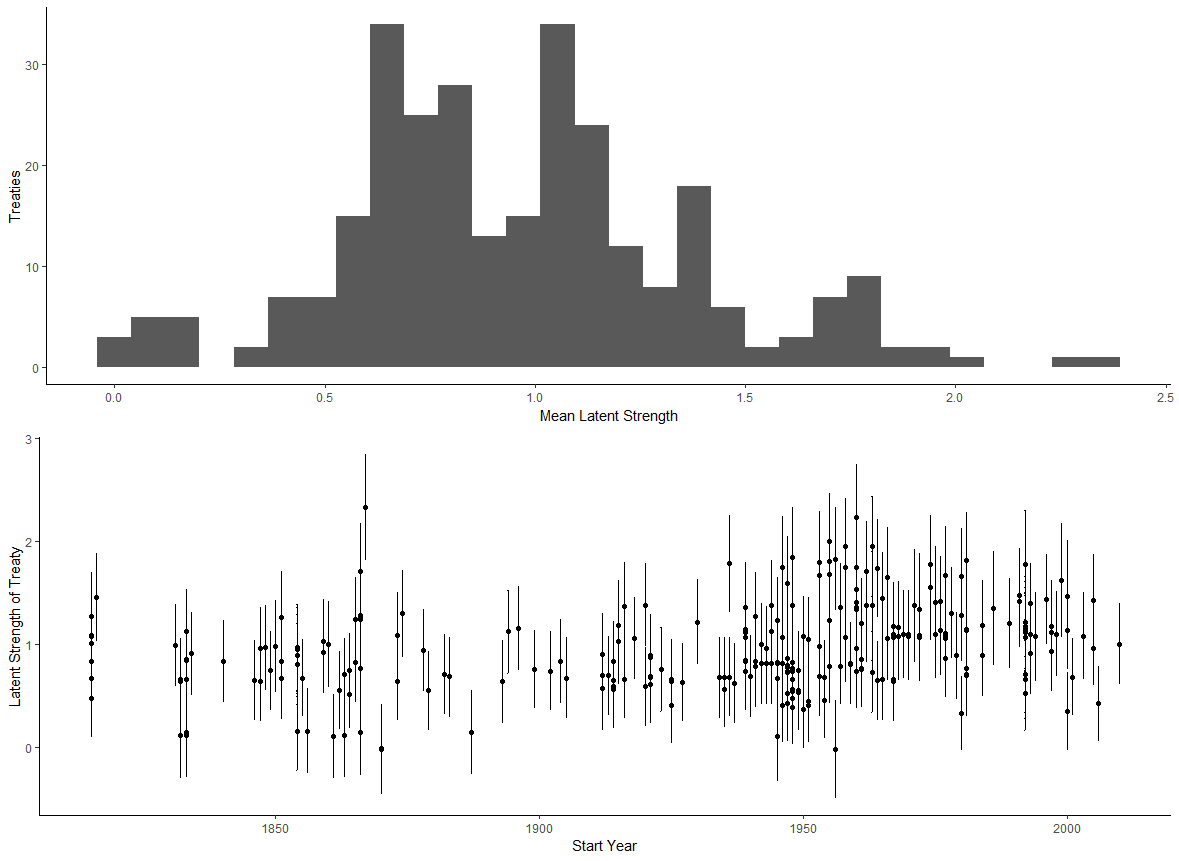
\includegraphics[width=0.95\textwidth]{../figures/ls-summary.png}
	\caption{Summary of latent measure of alliance treaty strength for 745 alliances from 1816 to 2016. The top panel is a histogram of the expected of alliance treaty strength. The bottom panel plots mean treaty strength (points) and the standard deviation (error bars) against the start year of the treaty.}
	\label{fig:ls-summary}
\end{figure}
	
	
The bottom panel of \autoref{fig:ls-summary} plots the posterior means and uncertainty in those estimates against the start year of the treaty. 
Even after accounting for posterior uncertainty, it is possible to distinguish between strong and weak treaties. 
Weak treaties are concentrated in the 20th century, when non-aggression and consultation alliances proliferated. 


% Cases- especially strong and weak treaties
The scale of the latent measure is not itself informative. 
The key information is differences in the latent measure between treaties. 
The mean of treaty strength is 0.01, and the median is -0.10. 
By this metric a 1938 consultation pact between France and Czechoslovakia (ATOPID 2120) is quite average. 


The weakest treaty is a neutrality and non-aggression treaty between Georgia and Kazakhstan (ATOPID 4476).  
A similar treaty between between Ukraine and India (ATOPID 4188) scores -1.36 on the latent measure.
The three strongest treaties are an 1867 alliance between Prussia and Hesse (ATOPID 1290), a 1955 treaty between Greece and Turkey governing relations in Cyprus and the United Arab Republic (ATOPID 3300).  
NATO, the best-known alliance, scores 0.75- so its formal promises are stronger than average, but not exceedingly strong. 
The weak treaties made few costly promises, while stronger treaties led to substantial concessions for members. 


This measure has face and discriminant validity. 
In this measure weak treaties had few sacrifices for participants. 
Also, the measurement model divides treaties into two distinct clusters of weak and strong commitments. 
Incorporating these changes in treaty strength and other variation among alliances is the key contribution of the multilevel model I use to estimate the association between treaty strength and members military spending.  


\subsection{Multilevel Model} 


% Best fit for theoretical process. Can compare alliances. 
Multilevel modeling combines standard approaches in the literature. 
Studies of specific alliances provide more detail, while general studies in panel data rely on coarse measures of alliance participation.
In this model, I estimate the impact of each alliance on member's military spending, but also the overall association between treaty strength and military expenditures. 
To overcome common estimation challenges, I fit this model in the Bayesian framework using STAN \citep{Carpenteretal2016}.\footnote{See the appendix for details of the weakly informative prior distributions and evidence of convergence.}


The multilevel model is more complex than traditional approaches. 
But added complexity has several benefits. 
First, multilevel modeling allows my test to match the theory. 
My predictions compare strong and weak treaties- and the alliance level regression in a multilevel model contains a corresponding coefficient.
Relying on a state-level proxy for alliance strength generates comparisons among states, which may produce misleading inferences. 


Last, multilevel modeling facilitates comparisons among alliances. 
The alliance-level regression controls for other alliance characteristics that are correlated with alliance strength and military spending.
Partial pooling allows me to estimate the unique impact of each alliance on members military spending. 
Comparing patterns in these alliance-specific coefficients provides additional evidence to examine Hypotheses 1 and 2 as well as the importance of treaty strength. 


% Two separate but connected regressions
% State-level regression- alliances enter through spending matrix.
This model contains two distinct but connected regressions. 
The base is a state-level regression, which is similar to a regular panel data model.
An alliance-level regression predicts parameters in the state-level regression, not unlike an interaction. 

The state-level regression can be expressed as:
\begin{equation}
y \sim student_t(\mu, \nu, \sigma)
\end{equation}
 
$y$ is the outcome of interest--- growth in military spending. 
I model growth in spending with a t-distribution to address large outliers in spending growth. 
$\mu$, the mean of the t-distributed outcome, is a function of several covariates. 
\begin{equation}
\mu = \alpha + \alpha^{st} + \alpha^{yr} + W \gamma + Z \lambda
\end{equation}


Growth in spending is a function of an overall intercept $\alpha$, state and year varying intercepts $\alpha^{st}$ and $\alpha^{yr}$, and a matrix of state-level control variables $W$. 
The $Z \lambda$ term adds alliance participation to the state-level model.


$Z$ is a matrix of state participation in alliances. 
Columns correspond to alliances, and rows with state-year observations. 
If a state is not part of an alliance, the corresponding cell of the matrix is zero.
If a state is part of an alliance in a given year, the corresponding cell of the matrix is the log of total allied military spending. 


I use total allied spending in the alliance participation matrix because how much capability a treaty provides shapes its value.   
Therefore, the $\lambda$ parameters capture alliance members' responsiveness to changes in allied capability. 
Each alliance has a unique $\lambda$, which come from a common distribution. 
These coefficients are a function of a second alliance-level regression. 

% Alliance-level regression:
The second part of the multilevel model uses alliance characteristics to predict how allied spending is associated with alliance members military spending. 
The $\lambda$ parameters are the dependent variable in an alliance-level regression, which includes alliance treaty strength.
Therefore, I focus interpretation on this second-level regression, where: 

\begin{equation}
\lambda \sim N(\theta, \sigma_{all})
\end{equation} 
and 
\begin{equation}
\theta = \alpha_{all} + \beta_1 \mbox{Treaty Strength} + X \beta
\end{equation}

% Like an interaction between alliance and state-level factors 
Hypothesis 1 predicts that $\beta_1$ will be negative among major powers, and Hypothesis @ predices that $\beta_1$ will be positive for non-major powers. 
In this alliance-level regression, $\textbf{X}$ is a matrix of alliance-level control variables and $\alpha_{all}$ is the constant.
Adding $\sigma_{all}$ means that the predictions of $\lambda$ are not deterministic--- the alliance level regression contains an error term. 
Coefficients in the alliance-level regression are like marginal effects in an interaction. 
A change in treaty strength modifies $\lambda$, which affects growth in military spending. 


% Provide an example observation
Consider one observation as an example of how the model works. 
Growth in Argentina's military spending in 1955 depends on Argentina's economic growth, political regime, conflict participation, and rivals. 
It is also affected by Argentine participation in the Rio Pact and OAS. 


\begin{equation}
\begin{split}
& \mbox{Argentina 1955} = \mbox{Overall mean}
+ \mbox{Argentine Intercept} + \mbox{1955 Intercept} 
+ \mbox{Argentine Characteristics} \\
& + \lambda_{OAS} * \mbox{OAS Expenditure} + \lambda_{Rio} * \mbox{Rio Pact Expenditure}
\end{split} 
\end{equation}


$\lambda_{OAS}$ and $\lambda_{Rio}$ are modified by the alliance level regression. 
The institutional design and membership of these treaties alter the $\lambda$ parameter.
Alliances that Argentina does not participate in have no impact on growth in military spending.  



\subsection{Sample and Covariates} 

% Sample of states and alliances: latter is restricted to treaties with military support 
I estimate this model on two sub-samples of states from 1816 to 2007. 
Alliance participation data comes from the ATOP project \citep{Leedsetal2002}. 
I focus on participation in defensive or offensive treaties, because it is hard to compare these treaties with consultation, neutrality or non-aggression pacts. 
Direct promises of military support give allied capability importance. 


% Because I think the DGP is different for large and small- split sample.
My argument suggests that major and non-major powers use alliances for different purposes.
Major powers focus on influence, non-major powers emphasize immediate territorial security.  
Therefore, the data-generating process connecting alliance participation and military spending should be different for these two states. 
To capture these differences, I estimate the model in separate samples- one sample of major powers, the other of non-major powers.
I employ the classification of major power status from the Correlates of War Project. 


The non-major power sample contains 8,668 observations. 
There are 930 major power observations. 
Though the major power sample is smaller and has fewer units, Bayesian estimation and partial pooling can generate plausible estimates \citep{Stegmueller2013}. 


% Describe covariates at each level. 
In the state-level regression, I control for several correlates of alliance participation and military spending. 
State-level covariates include GDP growth \citep{Boltetal2018}, regime type, international war \citep{Reiteretal2016}, civil war participation \citep{SarkeesWayman2010}, annual MIDs \citep{Gibleretal2016}, rival military spending \citep{ThompsonDreyer2012} and a dummy for Cold War years.
I include growth in GDP instead of levels of GDP because GDP levels are non-stationary, and economic growth shapes the opportunity costs of military spending \citep{Kimball2010, Zielinskietal2017}.
Alliance level variables include my measure of treaty strength, number of members and share of democracies at time of formation \citep{Chibaetal2015}, and whether the US or USSR participated in a treaty during the Cold War. 
Two dummy indicators of wartime alliances and asymmetric obligations \citep{Leedsetal2002} are also part of the alliance-level regression. 


Democratic membership in an alliance is associated both with limited obligations \citep{Chibaetal2015} and military spending \citep{DigiuseppePoast2016}, making it a particularly important alliance-level covariate.  
State and alliance-level controls for threat and conflict participation capture situations where states are more likely to seek allies. 
The next section describes the results from my research design. 

\section{Results}

% note on interpreting Bayesian results
Because I use Bayesian modeling to estimate the association between treaty strength and growth in military spending, there are no conventional indicators of statistical significance. 
Instead, each coefficient has a posterior distribution--- the possible values of the coefficient conditional on the prior and observed data. 
Thus I calculate the positive and negative posterior probability for the treaty strength coefficient to assess Hypotheses 1 and 2.


% show latent strength coefficient in each subset of data
\begin{figure}[htbp]
	\centering
		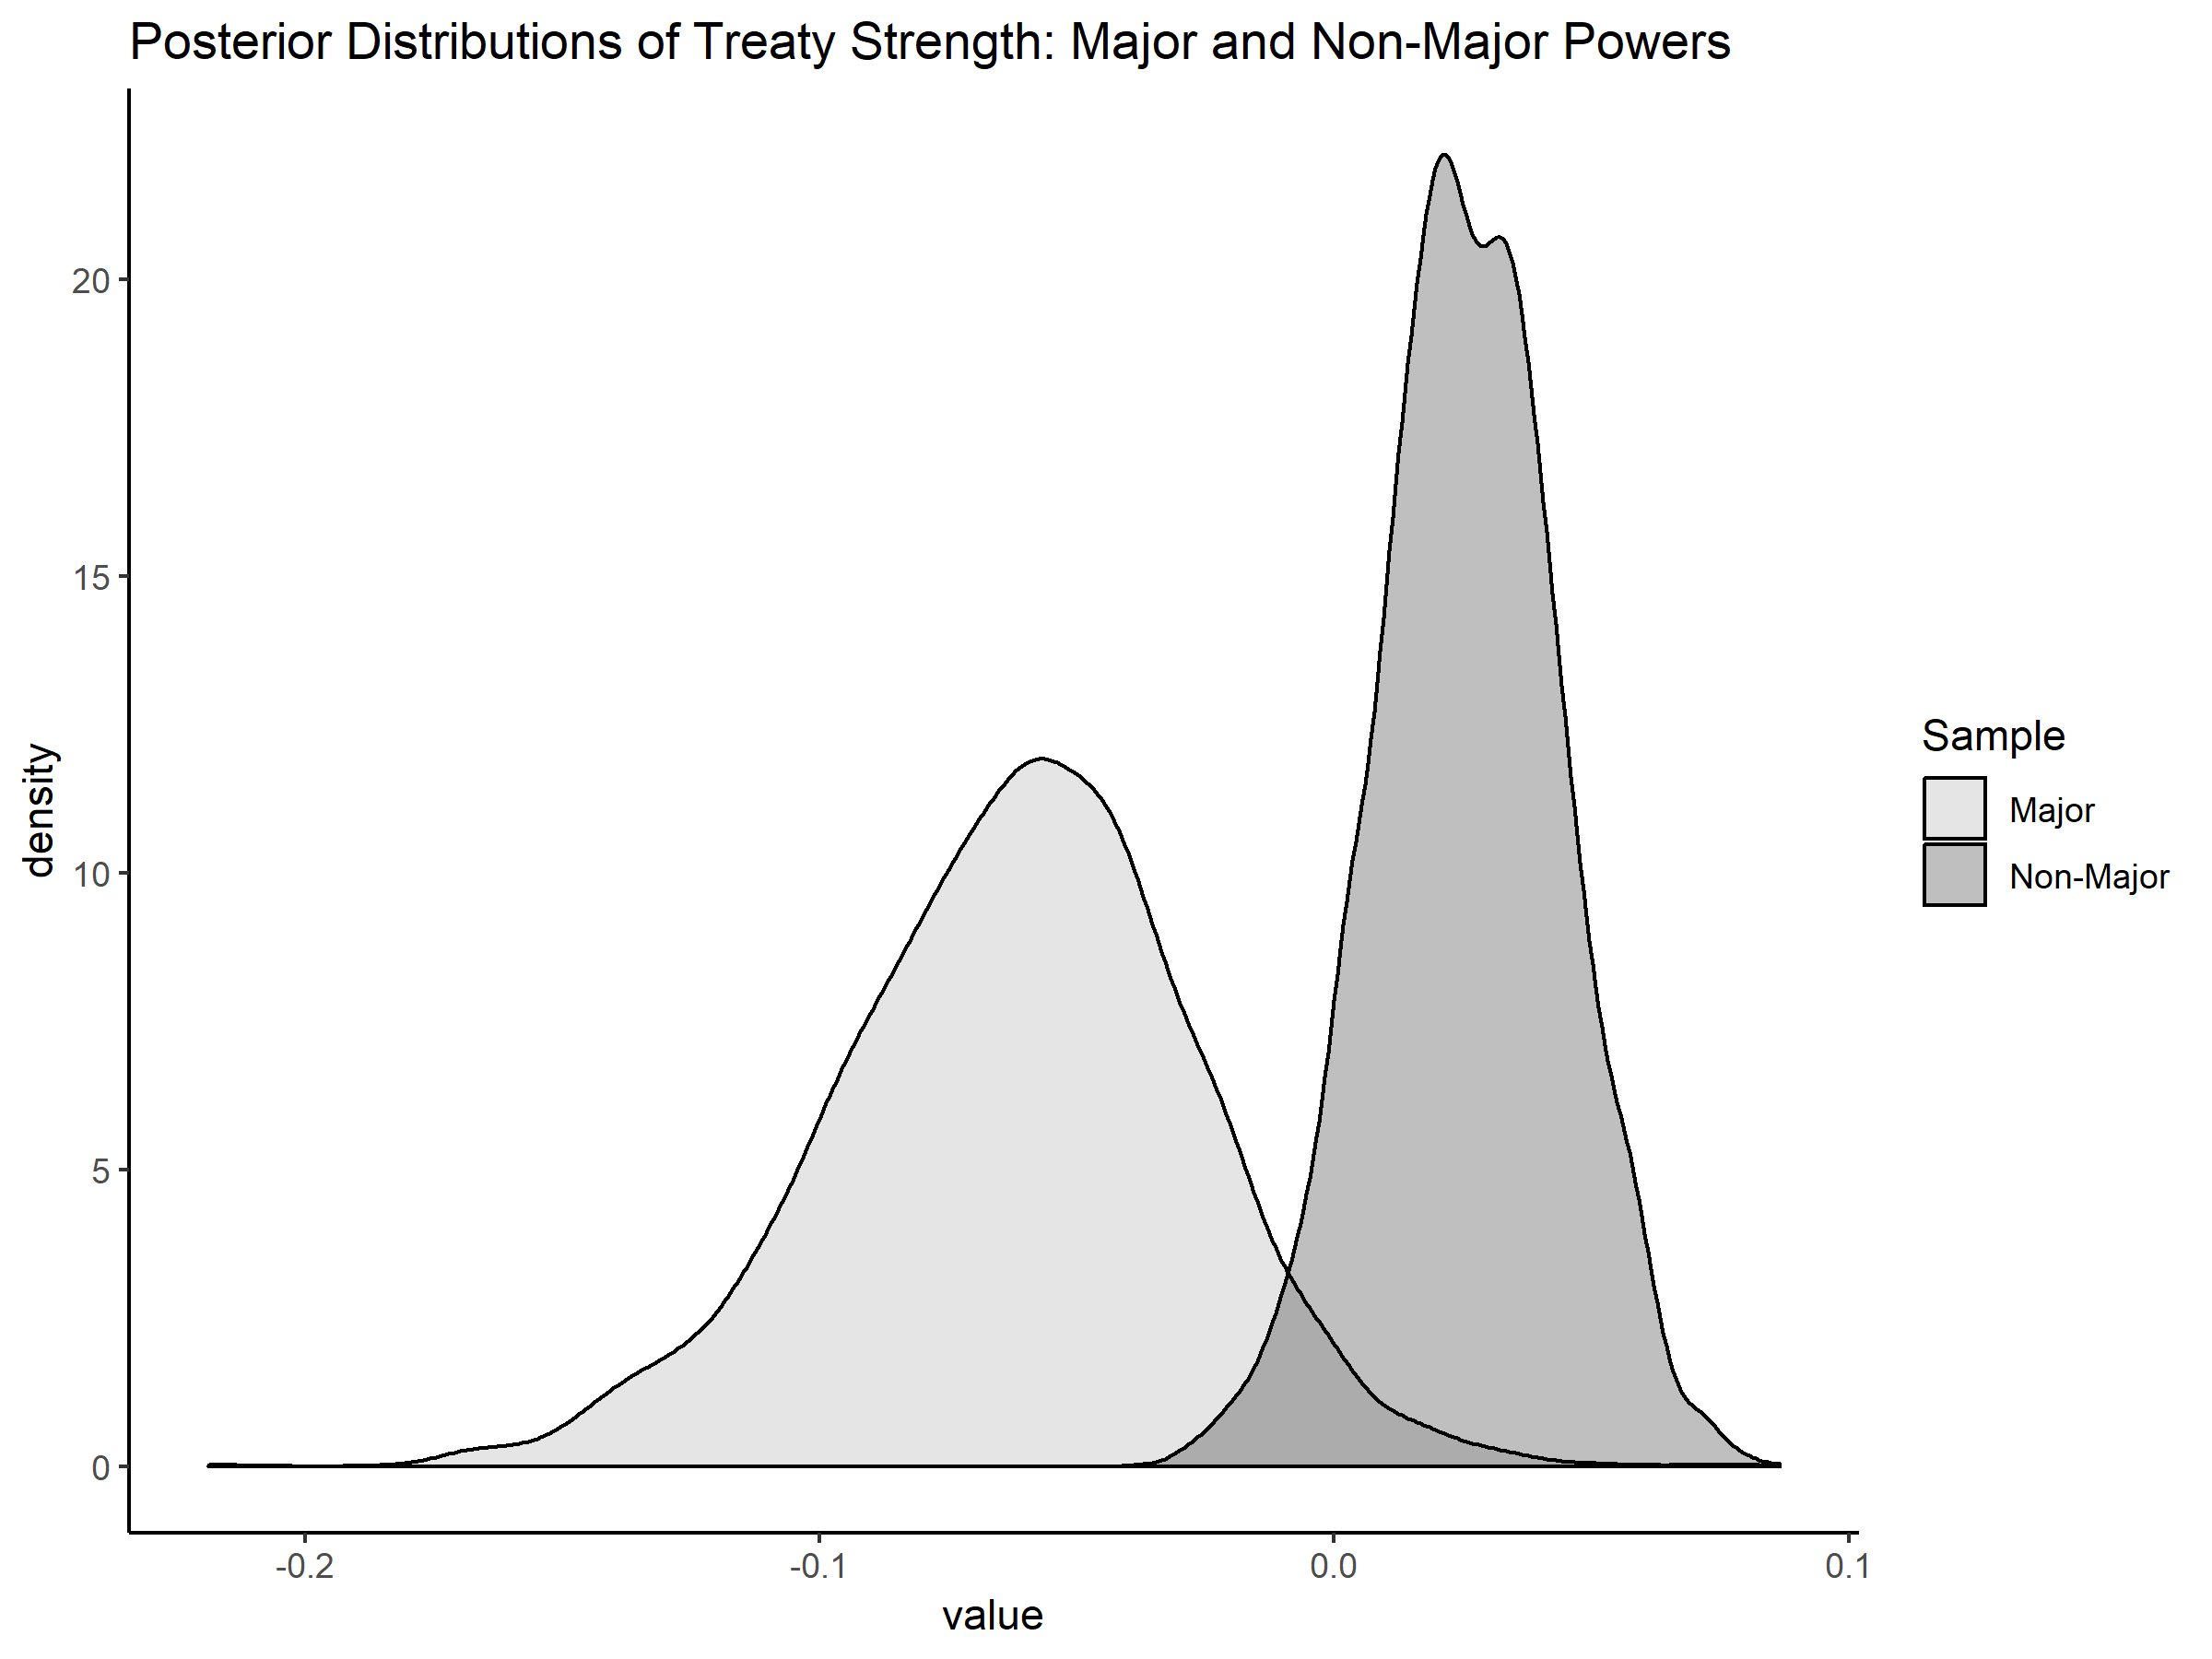
\includegraphics[width=0.95\textwidth]{../figures/str-dens.png}
	\caption{Posterior density of treaty strength coefficient in major and non-major power samples, 1816 to 2007. 96\% of the major power posterior mass is negative. 94\% of the non-major power posterior mass is positive.}
	\label{fig:str-dens}
\end{figure}


\autoref{fig:str-dens} plots the full posterior density of the treaty strength coefficients in the major and minor power samples. 
The smaller sample for major powers produces more variance in all the coefficient estimates. 
96\% of the posterior mass for major powers is negative. 
94\% of the posterior mass for minor powers is positive. 
There is little overlap between these two posteriors--- there is a 99\% chance that the association between treaty strength and military spending is larger for minor powers than major powers. 


These two coefficient estimates match the predictions of Hypotheses 1 and 2. 
For major powers, increasing treaty strength is associated with lower growth in military spending. 
Greater treaty strength is associated with higher growth in military spending for non-major powers.


How substantively important is treaty strength? 
Among major powers, the mean of the treaty strength coefficient is -0.05, and median growth in military expenditures is 0.04.\footnote{The median is a better summary of the dependent variable because large positive and negative outliers influence the mean.} 
So a one-unit increase in treaty strength offsets the typical annual growth in military spending. 


For non-major powers, the mean of the treaty strength coefficient is 0.03, and median growth in military expenditures is 0.06. 
Greater treaty strength increases growth in minor power military expenditures by about a third of typical growth. 
Increasing treaty strength has a large substantive effect, relative to the scale of the data. 
It also has a large influence on the overall association between changes in allied spending and growth in state defense spending. 


If greater treaty strength has a large influence on the $\lambda$ parameters, there will be a clear trend in the value of $\lambda$ across the range of alliance treaty strength.
We should observe a negative trend in the expected value of $\lambda$ as treaty strength increases in major power alliances. 
Conversely, we should observe a positive trend in $\lambda$ for non-major power alliances. 


\begin{figure}[htbp]
	\centering
		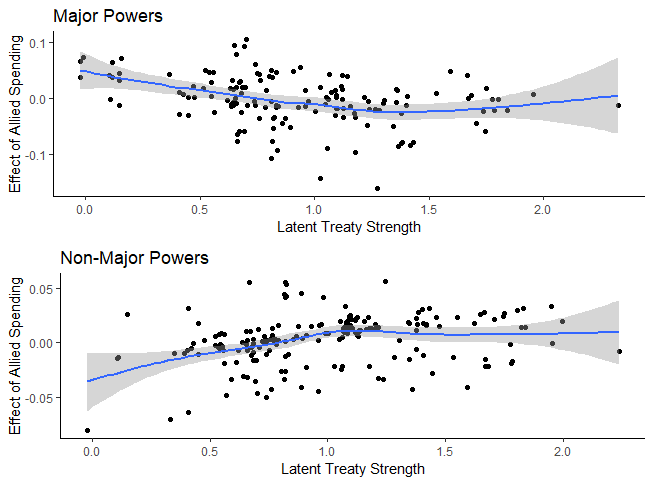
\includegraphics[width=0.95\textwidth]{../figures/lambda-ls-scatter.png}
	\caption{Scatter plots of trends in mean $\lambda$ parameters and treaty strength. Trend lines estimated using linear regression. }
	\label{fig:lambda-ls-scatter}
\end{figure}


\autoref{fig:lambda-ls-scatter} plots the expected value of the association between allied spending and state spending $\lambda$ against treaty strength in the two samples. 
In the major power sample, there is a slight negative trend in the scatter plot.
For non-major powers, the trend is positive. 
In both samples, the correlation between mean $\lambda$ and treaty strength is statistically significant. 


Because $\lambda$ captures the total impact of an alliance, this pattern suggests that increasing alliance strength has an important role. 
Even holding other alliance characteristics constant, alliance strength drives the overall effect of allied spending down for major powers, and up for non-major powers. 
Greater alliance treaty strength has the expected impact on military spending in strong and weak states. 


\section{Discussion}


% Matches argument 
The above results match the expectations of my argument. 
Increasing treaty strength is positively associated with growth in military spending in non-major powers, who use the greater freedom of action in weak treaties to rely on their partners. 
Greater treaty strength is associated with lower growth in military spending for major powers, who use treaty strength and military capability as substitutes while seeking influence. 


% Precise interpretation: compares strong and weak alliances. Not treaty vs absence. 
These results contribute to the debate over whether alliance participation increases or decreases military spending. 
Dissension between the force multiplier and foreign entanglement views of alliances is based on competing claims about the purposes of alliances. 
Some of these studies compare states in a particular kind of alliances to those outside the treaty. 
Others examine responsiveness to allied military spending. 


How do my results compare to previous evidence on alliance participation and military spending? 
The multilevel model reflects a conditional argument that is largely absent in prior studies. 
My key coefficient estimates compare strong and weak treaties, not states with a treaty to those without. 
However those estimates are like marginal effects- increasing treaty strength alters the effect of alliance participation.

 
$\lambda$ measures the impact of increasing allied spending \textit{for states in a treaty}. 
These parameters capture the impact of alliance participation only for treaty members. 
Therefore, a comparison between treaty members and non-members is included in the statistical model. 
Greater treaty strength makes the association between alliance participation and growth in military expenditures more negative for major powers, and more positive for non-major powers. 


My argument suggests claims that alliance participation only increases or decreases military spending are inappropriate. 
Instead, the association between alliance participation and growth in military spending depends on alliance member size and treaty strength. 
Alliance participation has heterogeneous effects because major powers and non-major powers employ treaties for different purposes. 
The conditional argument and research design show that alliance participation can increase or decrease spending for different states. 


% limitations of RD
There are several limitations to my research design.
First, measures of military spending are noisy and contain substantial measurement error. 
There is also a great deal of missing data in the 1816--2007 time frame of this study. 
I plan to check the robustness of my results to these issues in the near future by adding measurement error to the outcome and imputing of missing data.


The multilevel model only incorporates time-invariant alliance characteristics, save for changing capabilities in the membership matrix. 
So I measure share of democratic members and the number of members at time of formation. 
This is a relatively crude measurement strategy, and allowing time-varying alliance characteristics might improve the statistical model. 


% Strategic treaty design
Strategic alliance design is the last major weakness of the research design. 
Non-random selection into different kinds of alliances might lead to systematic differences between members that are not controlled for in my statistical model. 
I attempted to control for correlates of alliance treaty strength, especially democracy, but this is still a theoretical and empirical limitation. 



\section{Conclusion}


% Start conclusion 
This paper presented a novel argument and empirical evidence linking alliance participation and military expenditures. 
I explain when alliance participation is associated with greater military spending, and when it reduces growth in spending, bridging a debate between competing answers to this question. 
For major powers, greater treaty strength leads to lower growth in spending. 
Non-major power growth in spending increases in alliance treaty strength. 
I provide evidence for these predictions using a new measure of alliance treaty strength and a multilevel model. 


% Next steps: extend argument to other treaty characteristics
There are several next steps for research on the question. 
One is to extend the argument to other alliance characteristics. 
If major and non-major powers employ alliances for different ends, then other alliance characteristics may have different impacts on military spending. 
Large and small states might use wartime and asymmetric treaties differently, for instance. 


% Next steps: More interp of lambdas
Another task for future research is making more detailed comparisons of the $\lambda$ parameters for different alliances. 
Each $\lambda$ captures the aggregate impact of alliance participation.
As such, these parameters provide a novel measurement, and additional evidence of when alliance participation increases or decreases military spending. 


% Case studies
The multilevel model estimates do not establish causality. 
But the $\lambda$ parameters might provide a guide for selecting cases for a process-tracing analysis to corroborate the regression results.
One possible design is selecting the five largest and smallest $\lambda$ values for major and minor powers, and determining whether the connection between alliance participation and military expenditures matches the theoretical process.


% The argument indicates tradeoff
The argument and evidence suggests that major and non-major powers each face a tradeoff. 
Major powers tradeoff between the risk of entrapment and greater influence in strong treaties. 
Non-major powers sacrifice freedom of action for greater security as treaty strength rises. 


% Implications for policy. 
These twin tradeoffs have important consequences for policy debates.
The United States has a long history of decrying ``free-riding'' by allies who provide too little for their own defense \citep{Lanoszka2015}. 
But allies may be able to free-ride because the US prefers to form relatively weak alliance commitments. 
``Entangling alliances'' can provide greater influence to curb allied free-riding. 


Strong formal commitments can help restrain free-riding. 
The growing institutionalization of NATO, including the agreement for all allies to spend at least 2\% of GDP on defense, may reduce free-riding. 
However, conceptualizing alliances between major and non-major powers as the source of a public good is misleading. 
Asymmetric alliances produce different goods for different members. 
Major powers seek influence, while non-major powers secure their homeland. 


The US could also use stronger formal commitments as a substitute for greater defense effort in reassuring allies.
The danger is that making many strong commitments might create a situation where obligations exceed capabilities \citep{Kennedy1987}. 
Emboldening junior partners with a strong treaty might have deterrent value \citep{Bensonetal2014}, or increase the risk of conflict \citep{Benson2012}. 

 
% tie it all together
The connection between alliance participation and military expenditures depends on state size and the strength of the treaty.  
Alliance participation does not exclusively increase or decrease military spending.  
Both the force multiplier and foreign entanglement views of alliance participation are correct in different circumstances. 
Strong treaties have divergent effects on military spending in major and non-major powers. 



 
\bibliography{../../MasterBibliography} 





\end{document}
